
\documentclass[12]{article}

\usepackage{graphicx}
\usepackage{framed}
\usepackage{listings}
\usepackage{MnSymbol}
\usepackage{titlesec}
\usepackage{tikz}
\newcommand{\sectionbreak}{\clearpage}

\lstset{frame=tb,
  language=Java,
  aboveskip=3mm,
  belowskip=3mm,
  showstringspaces=false,
  columns=flexible,
  basicstyle={\small\ttfamily},
  numbers=none,
  breaklines=true,
  breakatwhitespace=true
  tabsize=3
}


\newtheorem{theorem}{Theorem}[section]
\newtheorem{lemma}[theorem]{Lemma}
\newtheorem{proposition}[theorem]{Proposition}
\newtheorem{corollary}[theorem]{Corollary}

\newenvironment{proof}[1][Proof]{\begin{trivlist}
\item[\hskip \labelsep {\bfseries #1}]}{\end{trivlist}}
\newenvironment{definition}[1][Definition]{\begin{trivlist}
\item[\hskip \labelsep {\bfseries #1}]}{\end{trivlist}}
\newenvironment{example}[1][Example]{\begin{trivlist}
\item[\hskip \labelsep {\bfseries #1}]}{\end{trivlist}}
\newenvironment{remark}[1][Remark]{\begin{trivlist}
\item[\hskip \labelsep {\bfseries #1}]}{\end{trivlist}}



\newcommand{\qed}{\nobreak \ifvmode \relax \else
      \ifdim\lastskip<1.5em \hskip-\lastskip
      \hskip1.5em plus0em minus0.5em \fi \nobreak
      \vrule height0.75em width0.5em depth0.25em\fi}
\newcommand{\pre}{\mathop{\mathrm{pre}}}
\newcommand{\myparagraph}[1]{\paragraph{#1}\mbox{}\\}





\begin{document}

\tableofcontents
\section*{Abstract}

\section{Introduction}

\begin{itemize}
\item Importance of autonomous systems and their verification
\item The state explosion problem, summary of different approaches
\item Our idea and contributions
\item Project objectives
\end{itemize}

\section{Background}

\subsection{Logics for Multi-Agent Systems}

\subsubsection{Multi-Agent Systems}

Autonomous multi-agent systems are computer systems which are made up of several intelligent ``agents" acting within an ``environment". 
Intuitively, an \textit{agent} is: 
\begin{itemize}
\item Capable of \textit{autonomous} action 
\item Capable of \textit{social} interaction with its peers
\item Acting to \textit{meet} their design objectives 
\end{itemize}
 
Suppose we have a multi-agent systems consisting of $n$ agents and an environment $e$.
\begin{definition} 
An agent $i$ in the system consists of: 
\begin{itemize}
\item A set $L_i$ of local states representing the different configurations of the agent,
\item A set $Act_i$ of local actions that the agent can take,
\item A protocol function $P_i : L_i \rightarrow 2^{Act_i} $ expressing the decision making of the agent.
\end{itemize} 
\end{definition}

We can define the environment $e$ as a similar structure $(L_e, Act_e, P_e)$ where $P_e$ represents the functioning conditions of the environment. 

\subsubsection{Interpreted Systems}
\label{IS}
We present a formal structure to represent multi-agent systems. Consider a multi-agent system $\Sigma$ consisting of $n$ agents $1, ..., n$ and an environment $e$.
\begin{definition}
An \textit{Interpreted System} $IS$ for $\Sigma$ is a tuple $(G, \tau, I, \sim_1, ..., \sim_n, \pi)$, where
\begin{itemize}
\item $G \subseteq L_1 \times ... \times L_n \times L_e$ is the set of global states that $\Sigma$ can reach. A global state $g \in G$ is essentially a picture of the system at a given point in time, and the local state of agent $i$ in $g$ is denoted $l_i(g)$.
\item $I \subseteq G$ is a set of intial states for the system
\item $\tau : G \times Act \rightarrow G $ where $Act = Act_1 \times ... \times Act_n \times Act_e$ is a deterministic transition function (we can define $\tau : G \times Act \rightarrow 2^G$ to model a non-deterministic system)
\item $\sim_1, ..., \sim_n \subseteq G \times G$  are binary relations defined by $$g \sim_i g' \Leftrightarrow l_i(g) = l_i(g') \quad \forall g, g' \in G, \forall i = 1, ..., n$$
i.e iff agent $i$ is in the same state in both $g$ and $g'$. 
\item $\pi : PV \rightarrow G$ is a valuation function for the set of atoms $PV$, i.e for each atom $p \in PV$, $\pi(p)$ is the set of global states where $p$ is true
\end{itemize}
\end{definition}

We also need a formal definition for the ``execution'' of a system. A \emph{run}, as defined below, represents one possible execution of a MAS. 
\begin{definition} 
A \emph{run} of an interpreted system $IS = (G, \tau, I, \sim_1, ..., \sim_n, \pi)$ is a sequence $r = g_0, g_1, ...$ where $g_0 \in I$ and such that for all $i \geq 0$, $\exists a \in Act$ such that $\tau(g_i, a) = g_{i+1}$.
\end{definition}

Interpreted Systems as defined above are used as semantic structures for a particular family of logics, presented in the next section.

\subsubsection{Linear Temporal Logic} 
\label{LTL}

In order to verify properties of multi-agent systems, we first need to find a logic allowing us to describe these properties accurately. 

A good candidate is the Linear Temporal Logic (LTL), a modal temporal logic in which one can write formulas about the future of \emph{paths}. Here we use paths to represent infinite runs of an interpreted system. 

\begin{definition} 
The syntax of LTL formulas is given by the following BNF: 
$$\varphi := p \mid \lnot\varphi \mid \varphi \land \varphi \mid X\varphi \mid G\varphi \mid \varphi U\varphi$$
\end{definition}

The intuitive meanings of $X\varphi, G\varphi$ and $\varphi U\psi$ are respectively 
\begin{itemize} 
\item $\varphi$ holds at the ne\textbf{X}t time instant
\item $\varphi$ holds forever (\textbf{G}lobally)
\item $\varphi$ holds \textbf{U}ntil $\psi$ holds  
\end{itemize}

We define the unary operator $F$ to be the dual of $G$, i.e $F\varphi := \lnot G\lnot\varphi$ for any LTL formula $\varphi$. $F\varphi$ represents the idea that $\varphi$ will hold at some point in the \textbf{F}uture.   

\myparagraph{Semantics} 

A model for LTL is a Kripke model $M = (W, R, \pi)$ such that the relation $R$ is serial, i.e $\forall u \in W,  \exists v \in W$ such that $(u, v) \in R$.
The worlds in $W$ are called the \textit{states} of the model. 

\begin{definition} 
A \textit{path} in an LTL model $M = (W, R, \pi)$ is an infinite sequence of states $\rho = s_0, s_1, ...$ such that $(s_i, s_{i+1}) \in R$ for any $i \geq 0$.
We denote $\rho^i$ the suffix of $\rho$ starting at $i$ (note that $\rho^i$ is itself a path since $\rho$ is infinite).
\end{definition}

It is easy to see how such a model can be used to represent a computer system, and how an execution of this system can be written as a path.

 Our objective is to be able to verify that a system $S$ has property $P$, so if we encode $P$ as an LTL formula $\varphi_P$ and $S$ as a model $M_S$, then we need to be able to check whether $\varphi_P$ is \textit{valid} in $M$ (or at least true in a set of initial states). This technique is called \textit{model checking}, and we do this by using the following definition for the semantics of LTL:
\label{model_checking}

\begin{definition}
Given LTL formulae $\varphi$ and $\psi$, a model $M$ and a state $s_0 \in W$, we say that
\begin{eqnarray*}
(M, s_0) \models p &\Leftrightarrow& s_0 \in \pi(p) \\  
(M, s_0) \models \lnot \varphi &\Leftrightarrow& (M, s_0) \nmodels \lnot \varphi\\
(M, s_0) \models \varphi \land \psi &\Leftrightarrow& (M, s_0) \models \varphi \mbox{ and  } (M, s_0) \models \psi \\
(M, s_0) \models X\varphi &\Leftrightarrow& (M, s_1) \models \varphi \mbox{  for all states } s_1 \mbox{ such that } R(s_0, s_1)\\
(M, s_0) \models G\varphi &\Leftrightarrow& \mbox{for all paths } \rho = s_0, s_1, s_2, ... , \mbox{ we have } (M, s_i) \models \varphi \quad \forall i \geq 0 \\
(M, s_0) \models \varphi U\psi &\Leftrightarrow& \mbox{for all paths } \rho = s_0, s_1, s_2, ..., \exists j \geq 0 \mbox{ such that }  (M, s_j) \models \psi \\ && \mbox{ and }  (M, s_k) \models \varphi \quad \forall 0 \leq k < j
\end{eqnarray*}

\end{definition}

The expressive power of LTL is limited to quantification over \textit{all} possible paths. For example: 

\begin{itemize}
\item $FG($deadlocked$)$ 

In every possible execution, the system will be permanently deadlocked.

\item $GF($crash$)$

Whatever happens, the system will crash infinitely often.
\end{itemize}

Hence some properties cannot be expressed in LTL, as in certain applications we might want to quantify explicitely over paths. The Computation Tree Logic (CTL) can express this. 

\subsubsection{Computation Tree Logic} 

\begin{definition} 
The syntax of CTL formulae is defined as follows: 
$$ \varphi := p \mid \lnot \varphi \mid \varphi \land \varphi \mid EX\varphi \mid EG\varphi \mid E(\varphi U \varphi)$$
\end{definition}

Intuitively, $ EX\varphi,  EG\varphi,$ and $ E(\varphi U \psi)$ represent the fact that there exists a possible path starting from the current state such that, respectively, $\varphi$ is true at the next state, $\varphi$ holds forever in the future, and $\varphi$ holds until $\psi$ becomes true.

The dual operator $AX\varphi := \lnot EX \lnot\varphi $ can be used to represent the fact that in all possible paths from the current state, $\varphi$ is true at the next state.
Connectives $AG\varphi, AF\varphi,$ and $A(\varphi U\psi)$ can be defined in the same way. 

We also use models (as defined in \ref{LTL}) for the semantics of CTL, as follows:

\begin{definition} 
Given CTL formulas $\varphi$ and $\psi$, a model $M = (W, R, \pi)$ and a state $s_0 \in W$, the satisfaction of formulas at $s_0$ in $M$ is defined inductively as follows: 
\begin{eqnarray*}
(M, s_0) \models p &\Leftrightarrow& s_0 \in \pi(p) \\  
(M, s_0) \models \lnot \varphi &\Leftrightarrow& (M, s_0) \nmodels \lnot \varphi\\
(M, s_0) \models \varphi \land \psi &\Leftrightarrow& (M, s_0) \models \varphi \mbox{ and  } (M, s_0) \models \psi \\
(M, s_0) \models EX\varphi &\Leftrightarrow& \exists \mbox{ a path } s_0, s_1, s_2, ... \mbox{ such that } (M, s_1) \models \varphi \\
(M, s_0) \models EG\varphi &\Leftrightarrow& \exists \mbox{ a path } s_0, s_1, s_2, ... \mbox{ such that } (M, s_i) \models \varphi \quad \forall i \geq 0\\
(M, s_0) \models E(\varphi U\psi) &\Leftrightarrow&  \exists \mbox{ a path } s_0, s_1, s_2, ... \mbox{ for which } \exists i \geq 0 \mbox{ such that }  (M, s_i) \models \psi \\ && \mbox{ and }  (M, s_j) \models \varphi \quad \forall 0 \leq j < i
\end{eqnarray*}
\end{definition}

The quantifiers allow for more properties to be expressed, for example:
\begin{itemize}
\item From any state it is possible to reboot the system.

$AGEX($reboot$)$ \quad (not expressible in LTL)

\item example 2


\end{itemize}

Again, some formulas can be expressed in LTL but not in CTL. For instance, the property that \textit{in every path where $p$ is true at some point then $q$ is also true at some point} is expressed in LTL as $Fp \rightarrow Fq $ but there is no equivalent CTL formula.
 The logic CTL* combines the syntax of LTL and CTL to provide a richer set of connectives. We will not go into any more details regarding CTL*, but we refer the reader to TODO for more information. 

\subsubsection{The Epistemic Logic CTLK}

In the case of multi-agent systems, we are interested in describing the system in terms of individual agents, and in particular their \textit{knowledge}. 

For this reason, we add a family of unary operators $K_i$ for $i = 1, ..., n$ to the modal connectives defined previously. Each $K_i$ will represent the intuitive notion of knowledge for agent $i$. 
This enables us to define the temporal-epistemic logics LTLK and CTLK, which are extensions of LTL and CTL, respectively. Here we leave out details about LTLK, as the practical applications we present later on only support CTLK. 



\begin{definition} 
The syntax of CTLK is defined by the following BNF: 
$$ \varphi := p \mid \lnot \varphi \mid \varphi \land \varphi \mid EX\varphi \mid EG\varphi \mid E(\varphi U \varphi) \mid  K_i\varphi \quad (i \in \{1, ..., n\})$$
\end{definition}  

We use interpreted systems (\ref{IS}) as semantic structures for CTLK. The satisfaction of a CTL formula on an interpreted system $IS$ is defined analogously to its satisfaction on a model $M$ whose worlds $W$ are the global states of $IS$, and whose relation function $R$ is the global transition function of $IS$. 
For example, $(IS, g_0) \models EX\varphi \mbox{  iff there is a run } r = g_0, g_1, g_2, ... \mbox{ of $IS$ such that } (IS, g_1) \models \varphi$.

The following definition completes the semantics of CTLK formulae:

\begin{definition}
Given an interpreted system $IS$, a global state $g$, an agent $i$ of $IS$, and a CTLK formula $\varphi$, we define
$$(IS, g) \models K_i \varphi \mbox{  iff  } \forall g' \in G, g \sim_i g' \Rightarrow (IS, g') \models \varphi$$

The connective $K_i$ expresses that agent $i$ \emph{knows} of the property $\varphi$ when the system's global state is $g$.

We extend the syntax and semantics of CTLK by adding two extra unary operators: $E$ (Everybody knows) and $C$ (Common knowledge), whose semantics are defined as follows:

\begin{eqnarray*}
(IS, g_0) \models E\varphi &\Leftrightarrow& (IS, g_0) \models K_i \varphi \quad \forall i = 1, ..., n \\
(IS, g_0) \models C\varphi &\Leftrightarrow&  (IS, g_0) \models \bigwedge^\infty_{k = 1} E^{(k)}\varphi \quad \\&& \mbox{ where } E^{(1)} = E \mbox{ and } E^{(j+1)} = EE^{(j)} \quad \forall j \geq 1
\end{eqnarray*}
\end{definition}


\subsection{Model Checking}

Model checking was briefly introduced in \ref{model_checking} as a automated verification technique, which can be used to check that a system $S$ satisfies a specification $P$. The technique involves representing $S$ as a logic system $L_S$ which captures all possible computations of $S$, and encoding the property $P$ as a temporal formula $\varphi_P$. 

The problem of verifying $P$ is then reduced to the problem of checking whether $L_S \vdash \varphi_P $. But we can now build a Kripke model $M_S = (W_S, R_S, \pi)$ such that $L_S$ is sound and complete over (the class of) $M_S$, so that $$L_S \vdash \varphi_P \Leftrightarrow M_S \models \varphi_P .$$ 
$M_S$ is the Kripke model representing all possible computations of $S$, i.e. $W_S$ contains all the possible computational states of the system and the relation $R_S$ represents all temporal transitions in the system. 

In the case of a multi-agent system as defined above, encoding $S$ as an interpreted systems of agents will satisfy the equivalence. 

\subsubsection{Explicit Model Checking}

\label{explicit}
In this section we introduce a basic approach to model checking, the so-called \textit{explicit} approach.

Suppose that we want to check that a multi-agent system $\Sigma$ satisfies a propery $P$. If $IS$ is an interpreted system representing $\Sigma$, and $\varphi$ the CTLK formula corresponding to $P$, we need to verify that $(IS, s_0) \models \varphi$, for all initial states $s_0 \in I$.

Algorithmically it is more efficient \cite{need ref} to compute the set of global states $[\varphi]$ of $IS$ where $\varphi$ is true, and check that $I \subseteq [\varphi]$. 
The following algorithm returns $[\varphi]$ for any CTLK formula $\varphi$.


\begin{lstlisting}[mathescape]

function SAT($\varphi$) 
// returns $[\varphi]$
if $\varphi = \top$: return $G$
if $\varphi = \bot$: return $\varnothing$
if $\varphi = p$: return $\pi(p)$ 
if $\varphi = \lnot\varphi_1$: return $G \setminus$SAT($\varphi_1$)
if $\varphi = \varphi_1\land\varphi_2$: return SAT($\varphi_1$)$\cap$SAT($\varphi_2$)
if $\varphi = EX\varphi_1$: return SAT$_{\mbox{EX}}(\varphi_1)$
if $\varphi = AF\varphi_1$: return SAT$_{\mbox{AF}}(\varphi_1)$
if $\varphi = E(\varphi_1 U\varphi_2 )$: return SAT$_{\mbox{EU}}(\varphi_1, \varphi_2)$
if $\varphi = K_i\varphi_1$: return SAT$_{\mbox{K}}(i, \varphi_1)$
if $\varphi = E\varphi_1$: return SAT$_{\mbox{E}}(\varphi_1)$
if $\varphi = C\varphi_1$: return SAT$_{\mbox{C}}(\varphi_1)$
end
$\\$
\end{lstlisting}

Notice that this covers all formulae $\varphi$, as $\{EX, AF, EU, K_i, E, C\}$ is a minimum set of connectives for CTLK. The respective auxilliary functions are defined below. Notation: for any global states $g_0, g_1$ of $IS$ we write $g_0 \rightarrow g_1$ iff $\exists a \in Act$ such that $\tau(g_0, a) = g_1$ (i.e. there is an run of $IS$ starting with $g_0, g_1, ...$).


\begin{lstlisting}[mathescape]

function SAT$_{\mbox{EX}}$($\varphi$)
// returns $[EX\varphi]$
  X := {$g_0 \in G \mid g_0 \rightarrow g_1$ for some $g_1 \in $SAT($\varphi$) }
  return X
end
 
function SAT$_{\mbox{AF}}$($\varphi$)
// returns $[AF\varphi]$
  X := $G$
  Y := SAT($\varphi$)
  repeat until X = Y:
    X := Y
    Y := Y $\cup$ $\{ g_0 \in G \mid $ for all $g_1 $ with $g_0 \rightarrow g_1$, $g_1 \in$ Y $\}$ 
  end
  return Y
end
  

function SAT$_{\mbox{EU}}$($\varphi_1$, $\varphi_2$)
// returns $[E(\varphi_1U\varphi_2)]$
  W := SAT($\varphi$)
  X := $G$
  Y := SAT($\psi$)
  repeat until X = Y:
    X := Y
    Y := Y $\cup$ (W $\cap$ $\{g_0 \in G \mid \exists g_1 \in$ Y such that $g_0 \rightarrow g_1\}$)
  end
  return Y
end

function SAT$_{\mbox{K}}$($i$, $\varphi$)
// returns $[K_i\varphi]$
  X := SAT($\lnot\varphi$)
  Y := $\{g_0 \in G \mid \exists g_1 \in$ X with $R_i(g_0, g_1)\}$
  return $G \setminus\mbox{Y}$
end

function SAT$_{\mbox{E}}$($\varphi$)
// returns $[E\varphi]$
  X := SAT($\lnot\varphi$)
  Y := $\{g_0 \in G \mid \exists g_1 \in$ X with $R_i(g_0, g_1)$ for all $i = 1, ..., n\}$
  return $G \setminus\mbox{Y}$
end

function SAT$_{\mbox{C}}$($\varphi$)
// returns $[C\varphi]$
  X := $G$
  Y := SAT($\lnot\varphi$)
  repeat until X = Y:
    X := Y
    Y := $\{g_0 \in G \mid \exists g_1 \in$ X with $R_i(g_0, g_1)$ for all $i = 1, ..., n\}$
  end
  return $G \setminus\mbox{Y}$
end

\end{lstlisting}

TODO write something about $R_i$. 

The complexity of \texttt{SAT} is linear in the size of the model. However, the size of the model grows exponentially in the number of variables used to describe the system $\Sigma$, therefore the explicit approach is not always viable in practice. This is the main difficulty in model checking and it is known as the \textit{state explosion problem}. 

In the next section we introduce a model checking technique aiming to improve the efficiency of the approach. 

\subsubsection{Symbolic Model Checking}

\textit{Symbolic model checking} is an approach to model checking which involves representing sets of states and functions between them as Boolean formulas. The algorithm presented in \ref{explicit} is then reduced to a series of operations on Boolean formulas. In this section we go through the process of encoding sets and functions as propositional formulas, and we explain how this encoding facilitates model checking.

\myparagraph{Symbolic Representation of Sets of States}
\label{symbolic}
\begin{figure}
    \centering
    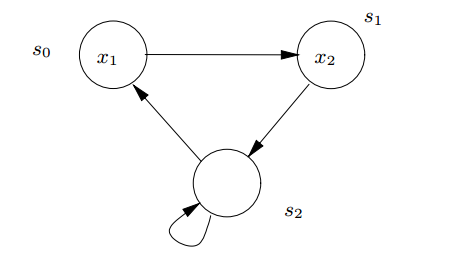
\includegraphics[scale=0.55]{symbolic_model_checking_example.PNG}
    \caption{A model}
    \label{fig:model_example}
\end{figure}

The encoding process is best illustrated by an example  \cite{logic_in_computer_science}
Consider the model in Figure~\ref {fig:model_example}, representing a system with three states labelled $s_0, s_1, s_2$. 

We consider two propositional variables, namely $x_1$ and $x_2$.  
If $S$ is the whole state space (so $S = \{s_0, s_1, s_2\}$), we can represent subsets of $S$ using Boolean formulae, as shown in the following table:\\

\begin{tabular}{ l | r }
  set of states & representation by boolean formula \\ \hline
$\emptyset $&   $\bot$ \\
$\{ s_0\}$ & $x_1 \land \lnot x_2 $\\
$\{ s_1\}$ & $ \lnot x_1 \land x_2 $\\
$\{ s_2\}$ & $\lnot x_1 \land \lnot x_2 $\\
$\{ s_0, s_ 1\}$ & $(x_1 \land \lnot x_2) \lor (\lnot x_1 \land x_2)  $\\
$\{ s_1, s_2\}$ & $(\lnot x_1 \land  x_2) \lor (\lnot x_1 \land\lnot x_2)$\\
$\{ s_0, s_2\}$ & $(x_1 \land \lnot x_2) \lor (\lnot x_1 \land\lnot x_2) $\\
$\{ s_0, s_1, s_2\}$ & $(x_1 \land \lnot x_2) \lor (\lnot x_1 \land  x_2) \lor (\lnot x_1 \land\lnot x_2)$
\end{tabular}
\\
\\

Note that for this representation to be unambiguous, we must ensure that no two states satisfy the same set of Boolean variables. If this is the case, new variables can be added which will be used to differenciate between the ambiguous states.

\myparagraph{Symbolic Representation of the Transition Relation}

The transition relation $\rightarrow$ of a model is a subset of $S \times S$. Taking two copies of our set of propositional variables, we can then associate a Boolean formula to the transition relation. In the example above, the transition relation $\rightarrow$ of the model is $\{(s_0, s_1), (s_1, s_2), (s_2, s_0), (s_2, s_2)\}$. 
Using our Boolean representations for $s_0, s_1$, and $s_2$, we compute the representation of $\rightarrow$ to be $$(\lnot x_1 \land \lnot x_2 \land \lnot x'_1 \land \lnot x'_2 ) \lor (\lnot x_1 \land \lnot x_2 \land x'_1 \land \lnot x'_2 ) \lor ( x_1 \land \lnot x_2 \land \lnot x'_1 \land  x'_2 ) \lor (\lnot x_1 \land x_2 \land \lnot x'_1 \land \lnot x'_2 )$$

[needs more details on the computation]\\\\

How does this help us? Well, several techniques exist which allow us to represent these Boolean formulas in a very concise form. This is the topic of the next section.

\subsection{Representing Boolean functions}

It is important to make the point that the Boolean formulas computed in \ref{symbolic} can be regarded as Boolean \textit{functions}, i.e. functions $\{0, 1\}^n \rightarrow \{0, 1\}$ for some $n$. For example, the formula $x_1 \land \lnot x_2$ is associated to the function $f(x_1, x_2) = x_1 \land \lnot x_2$.

In this section we introduce a theory of representations of Boolean functions using directed acyclic graphs (DAG). 

\subsubsection{Ordered Binary Decision Diagrams}

After truth tables, one the most basic ways of representing Boolean functions is by using a \textit{binary decision tree} (BDT). A BDT is a binary tree where we label non-terminal nodes with Boolean variables $x_1, x_2, ...$ and terminal nodes with the values 0 and 1. Each non-terminal node has two outgoing edges, one solid and one dashed (one for each value of the variable the node is labelled with). An example is shown in Figure~\ref{fig:BDT}. Note that the initial ordering of the variables changes the resulting BDT; for convenience, we write $[x_1, x_2, ..., x_n]$ to denote the order $x_1 < x_2 < ... < x_n$.


BDTs are a relatively inefficient way of storing Boolean formulas, since a BDT for a formula with $n$ variables will have $2^{n+1} - 1$ nodes. Fortunately, a BDT can be reduced to an \textit{ordered binary decision diagram} (OBDD), a much more compact data structure.

\begin{figure}
\centering
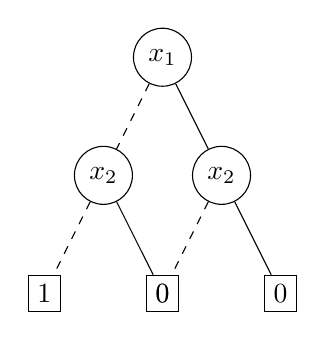
\begin{tikzpicture}

	[level 1/.style={sibling distance=33mm},
	 level 2/.style={sibling distance=23mm}]
	\node[circle, draw] (x1) {$x_1$}	 
		child {node[circle,draw] (x21) {$x_2$} [dashed]
			child {node[rectangle, solid, draw] (1) {1} [dashed]}
			child {node[rectangle, solid, draw] (01) {0} [solid]}}
		child {node[circle,draw] (x22) {$x_2$} [solid]
			child {node[rectangle, solid, draw] (02) {0} [dashed]}
			child {node[rectangle, solid, draw] (03) {0} [solid]}};
\end{tikzpicture}
	\caption{BDT for $f(x_1, x_2) = x_1 \land \lnot x_2$ under the ordering $[x_1, x_2]$}
\label{fig:BDT}
\end{figure}

\myparagraph{The Reduction Algorithm} 

There are three steps in the reduction of BDTs to OBDDs:
\begin{enumerate}
\item Removal of duplicate terminals: we merge all the 0-nodes and 1-nodes into two unique terminal nodes
\item Removal of redundant tests: if both outgoing edges of a node $n$ point to the same node $m$, we remove $n$ from the graph, sending all its incoming edges directly to $m$ 
\item Removal of duplicate non-terminals: we merge any two subtrees with identical BDD structure
\end{enumerate}

Steps (2) and (3) are repeatedly applied until no further reduction is possible. The resulting diagram is said to be a ordered binary decision diagram. 

[here need example of using reduction algorithm]

The following key result makes the use of OBDDs viable in practice: 

\begin{theorem}
\label{obdd_uniqueness}
If $f$ is a Boolean function over the variables $x_1, ..., x_n$, then the OBDD representing $f$ is unique, up to the order of $x_1, ..., x_n$ chosen.
\end{theorem}

The immediate consequence of Theorem~\ref{obdd_uniqueness} is that one can easily compare two Boolean functions by comparing their respective OBDDs (provided both OBDDs have the same variable order). 

Another important observation to make is that OBDDs resulting from two different variable orders may present a \textit{significant }difference in size, and therefore a large amount of work has been done in the search for suitable variable orders. 

OBDDs help us to manipulate Boolean functions with a high number of variables, allowing us to use our model checking algorithm (\ref{explicit}) on systems with much larger state-spaces, which has led researchers in the past 15 years to explore various graph-based representations of Boolean functions.

\noindent\textit{Note to the reader: throughout this report we often drop the `O' and refer to OBDDs as BDDs.}

\subsubsection{Knowledge Compilation Map}

In computer science, the field of \textit{knowledge compilation} is concerned with finding compact and efficient representations of propositional knowledge bases (such as symbolic representations of state-spaces, cf \ref{symbolic}).
 Such a representation is refered to as a \textit{target compilation language}, of which BDTs and OBDDs are examples. 
 
 The main properties that we look for in a target compilation language are the canonicity of the representation, the succinctness of the representation, and a polynomial-time complexity for queries and operations on the language. 
 These properties will ensure that we can safely rely on a particular language for our model checking algorithm. 
 
 OBDDs satisfy these properties (with succintness remaining highly dependent on the variable order), and in fact a number of model checkers use them for state-space representation (e.g. NuSMV, MCMAS). 
 
 In 2002, A. Darwiche and P. Marquis published \ref{compilation_map} a comparative analysis of most existing DAG-based target compilation languages in terms of their succintness and the polytime operations they support. They show that all of these languages are a subset of a broad language called \textit{negation normal form} (NNF). 

\begin{definition}
A sentence in \textit{NNF} is a rooted directed acyclic graph where each leaf node is labelled with $\top$, $\bot$, $X$ or $\lnot X$ for some propositional variable $X$, and each internal node is labelled with $\land$ or $\lor$ and can have arbitrarily many children. 

\end{definition} 

\noindent Remark: OBDDs are NNF sentences. Figure~\ref{nnf_obdd} shows an OBDD and its corresponding NNF sentence.  

\begin{figure}
\centering
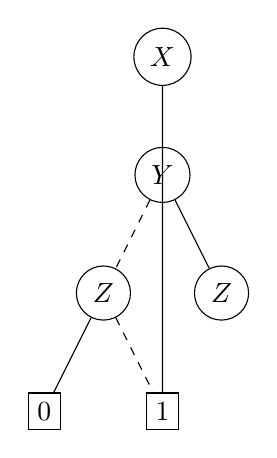
\begin{tikzpicture}

	[level 1/.style={sibling distance=33mm},
	 level 2/.style={sibling distance=23mm},
	 level 3/.style={sibling distance=16mm}]
	\node[circle, draw] (X) {$X$}	 
		child {node[circle, solid, draw] (Y) {$Y$} [dashed]
			child {node[circle, solid, draw] (Z1) {$Z$} [dashed]
				child {node[rectangle, solid, draw] (0) {0} [solid]}
				child {node[rectangle, solid, draw] (1) {1} [dashed]}}
			child {node[circle, solid, draw] (Z2) {$Z$} [solid]}};
	\draw[solid] (X) -- (1); 
\end{tikzpicture}
\qquad\quad
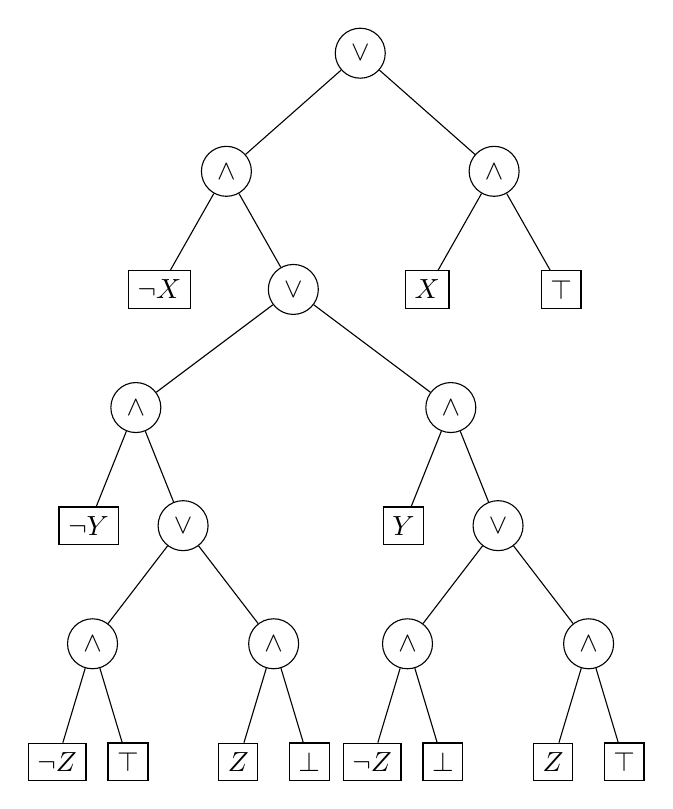
\begin{tikzpicture}
	[level 1/.style={sibling distance=34mm},
	 level 2/.style={sibling distance=17mm},
	 level 3/.style={sibling distance=40mm},
	 level 4/.style={sibling distance=12mm},
	 level 5/.style={sibling distance=23mm},
	 level 6/.style={sibling distance=9mm}]
	\node[circle, draw] (or1) {$\lor$}	 
		child {node[circle,draw] (and1) {$\land$} [solid]
			child {node[rectangle, solid, draw] (X1) {$\lnot X$}[solid]}
			child {node[circle, solid, draw] (or2) {$\lor$} [solid]
				child {node[circle,draw] (and3) {$\land$} [solid]
					child {node[rectangle, solid, draw] (Y1) {$\lnot Y$}[solid]}
					child {node[circle, solid, draw] (or5) {$\lor$} [solid]
						child {node[circle,draw] (and5) {$\land$} [solid]
							child {node[rectangle, solid, draw] (Z1) {$\lnot Z$}[solid]}
							child {node[rectangle, solid, draw] (T2) {$\top$} [solid]} 	
						}
						child {node[circle,draw] (and6) {$\land$} [solid]
							child {node[rectangle, solid, draw] (Z2) {$Z$}[solid]}
							child {node[rectangle, solid, draw] (F1) {$\bot$} [solid]} 	
						}
					}
				}
				child {node[circle,draw] (and4) {$\land$} [solid]
					child {node[rectangle, solid, draw] (Y2) {$Y$}[solid]}
					child {node[circle, solid, draw] (or6) {$\lor$} [solid]
						child {node[circle,draw] (and7) {$\land$} [solid]
							child {node[rectangle, solid, draw] (Z3) {$\lnot Z$}[solid]}
							child {node[rectangle, solid, draw] (F2) {$\bot$} [solid]} 	
						}
						child {node[circle,draw] (and8) {$\land$} [solid]
							child {node[rectangle, solid, draw] (Z2) {$Z$}[solid]}
							child {node[rectangle, solid, draw] (T2) {$\top$} [solid]} 	
						}
					}
				}
			}
		}
		child {node[circle,draw] (and2) {$\land$} [solid]
			child {node[rectangle, solid, draw] (X2) {$X$} [solid]}
			child {node[rectangle, solid, draw] (T1) {$\top$} [solid]}
		};
\end{tikzpicture}

	\caption{An OBDD (left) and its corresponding NNF sentence (right). Although the former seems much more compact, the difference in size is only linear and both representations are essentially the same. TODO sort this oout}
\label{nnf_obdd}

\end{figure}
 
 
 
\subsubsection{Project Directions}

 This ``knowledge compilation map" was the starting point for this project, whose initial objective was to investigate new target compilation languages suitable for application to model checking, seeking a potential improvement on BDDs (which constitute so far the ``industry standard").

 Taking into account the various criteria for suitable representations described above, we searched the literature aiming to find a good candidate to replace BDDs. 

After considering a number of different representations including trees-of-BDDs \ref{}, BDD-trees \ref{}, and several other subsets of NNF described in \ref{compilation_map}, we opted for a relatively novel target compilation language called \textit{sentential decision diagram} (SDD). 

SDDs are a subset of NNF, possess the required properties, and had not yet been experimented with in the context of model checking and state-space representation. 
Moreover, some of the experimental results presented in \ref{sdd1} and \ref{sdd2} demonstrate that SDDs can lead to a significant improvement on BDDs in terms of computation time and memory usage. 

In the next section we present SDDs in full details, delaying our own experimental results to the following chapters.


\subsection{Sentential Decision Diagrams}

\subsubsection{Preliminary Definitions}

To define SDDs formally we must start with some preliminary definitions related to Boolean functions. 

\begin{definition} 
Let $f$ be a Boolean function. If $X$ is a set of variables, the \textit{conditioning} of $f$ on an instantiation \textbf{x}, written $f|_{\textbf{x}}$ is the Boolean function obtained by setting variables of $f$ in $X$ to their value in \textbf{x}. 
We say that a function $f$ \textit{essentially depends} on a variable $x$ iff $f|_{x} \neq f|_{\lnot x}$, and we write $f(X)$ if $f$ essentially depends on variables in $X$ only.
\end{definition}

\noindent Notation: we also write $f(X, Y)$ if $f(Z)$ and $X$, $Y$ are sets forming a partition of $Z$.

The following definition is the basis for the construction of SDDs:

\begin{definition} (Decompositions and partitions)

An \textit{($X$,$Y$)-decomposition} of a function $f(X, Y)$ is a set of pairs $$\{(p_1, s_1),...,(p_n, s_n)\}$$ such that $$ f = (p_1(X) \land s_1(Y)) \lor ... \lor (p_n(X) \land s_n(Y)).$$
The decomposition is said to be \textit{strongly deterministic} on $X$ if $p_i(X) \land p_j(X) = \bot$ for $i \neq j$. In this case, each ordered pair $(p_i, s_i)$ in the decomposition is called an \textit{element}, each $p_i$ a \textit{prime} and each $s_i$ a \textit{sub}.

Let $\alpha = \{(p_1, s_1),...,(p_n, s_n)\}$ be an ($X,Y$)-decomposition, and suppose $\alpha$ is strongly deterministic on $X$.
Then $\alpha$ is called an $X$-\textit{partition} iff its primes form a partition (i.e primes are pairwise mutually exclusive, each prime is consistent, and the disjunction of all primes is valid.)
We say that $\alpha$ is \textit{compressed} if $s_i \neq s_j$ for $i \neq j$.
\end{definition}

\begin{example} 
Let $f(x, y, z) = (x \land y) \lor (x \land z)$. Then $\alpha = \{(x, y\lor z)\}$ is an $(\{x\}, \{y, z\})$-decomposition of $f$ which is strongly deterministic (as there is only one prime). It is however not an $\{x\}$-partition, but $\beta = \{(x, y\lor z), (\lnot x, \bot)\}$ is, since $x, \lnot x$ form a partition. Note that $\beta$ is compressed. 
\end{example}

\noindent Remark: Notice that in an $X$-partition $\bot$ can never be prime, and if $\top$ is prime then it is the only prime. Moreover primes determine subs, so two $X$-partitions are different iff they contain distinct primes.

\begin{theorem}
\label{theorem_apply}
Let $\circ$ be a Boolean operator and let $\{(p_1, s_1),...,(p_n, s_n)\}$ and $\{(q_1, r_1),...,(q_m, r_m)\}$  be $X$-partitions of Boolean functions $f(X, Y)$ and $g(X, Y)$ respectively. Then $$\{(p_i \land q_j, s_i \circ r_j) \mid  p_i \land q_j  \neq \bot \}$$ is an $X$-partition of $f \circ g$.
\end{theorem}
\begin{proof}
 Since $p_1, ..., p_n$ and $q_1, ..., q_m$ are partitions, the $(p_i \land q_j$ also form a partition for $i = 1, ..., n$, $j = 1, ..., m$ and $p_i \land q_j \neq \bot$. 
\end{proof}

As we see later on, an important consequence of Theorem~\ref{theorem_apply} is the polynomial time operations available on SDDs. Canonicity of SDDs is due to the following result:

\begin{theorem}
A function $f(\textbf{X}, \textbf{Y})$ has exaclty one compressed \textbf{X}-partition.
\end{theorem}
\begin{proof}
proof
\end{proof}

\myparagraph{Vtrees}

Vtrees (``variable trees") are to SDDs what variable orders are to BDDs. A vtree completely determines the structure of an SDD, so they are crucial to the viability of SDDs in practice.

\begin{definition}
A \textit{vtree} for variables $X$ is a full binary tree whose leaves are in one-to-one correspondence with the variables in $X$. We will often not distinguish between a vtree node $v$ and the subtree rooted at $v$, and the left and right children of a node $v$ will be denoted $v^l$ and $v^r$, respectively.
\end{definition}

\begin{example}
Let $X = \{x_1, x_2, x_3, x_4\}$. The following are two vtrees for $X$. 
\end{example}

Note that a vtree on \textbf{X} is stronger than a total order of the variables in \textbf{X}. Example \ref{test} shows two distinct vtrees which induce the same variable order. 

Now, let $f(\textbf{X})$ be a Boolean function and let $v$ be a vtree for \textbf{X}. We can construct an SDD for $f$ using a recursive algorithm, as follows.

 We first notice that variables in \textbf{X} are split into two disjoint sets, namely the variables in $v^l$ (say, \textbf{Y}) and the variables in $v^r$ (say, \textbf{Z}). Now, let $\alpha =  \{(p_1, s_1),...,(p_n, s_n)\}$ be a \textbf{Y}-partition of $f(\textbf{Y}, \textbf{Z})$. We apply this decomposition again to each prime 

[...] describe more
\subsubsection{Syntax and Semantics of SDDs}


\begin{definition} (Syntax)
Let $v$ be a vtree. $\alpha$ is an SDD that respects $v$ iff: 
\begin{itemize} 
\item $\alpha = \top$ or $\alpha = \bot$
\item $\alpha = X$ or $\alpha = \lnot X$, and $v$ is a leaf with variable $X$
\item $v$ is internal, and $\alpha$ is a partition  $\{(p_1, s_1), ..., (p_n, s_n)\}$ such that for all $i$, $p_i$ is an SDD that respects $v^l$ and $s_i$ is an SDD that respects $v^r$.
\end{itemize}
In the first two cases we say that $\alpha$ is \textit{terminal}, and in the third case $\alpha$ is called a \textit{decomposition}. For SDDs $\alpha$ and $\beta$, we write $\alpha = \beta$ iff they are \textit{syntactically equal}.
\end{definition}

\begin{definition} (Semantics)
Let $\alpha$ be an SDD. We use $\langle . \rangle$ to denote the mapping from SDDs to Boolean functions, and we define it inductively as follows: 
\begin{itemize} 
\item $\langle \top \rangle = \top$ and  $\langle \bot \rangle = \bot$
\item $\langle X \rangle = X$ and $\langle \lnot X \rangle = \lnot X$, for all variables $X$
\item $\langle\{(p_1, s_1), ..., (p_n, s_n)\}\rangle = \bigvee_{i = 1}^n \langle p_i \rangle \land \langle s_i \rangle  $
\end{itemize}
We say two SDDs $\alpha$ and $\beta$ are \textit{equivalent} (written $\alpha \equiv \beta$) if $\langle \alpha \rangle = \langle \beta \rangle$.

\end{definition}


\subsubsection{Construction of SDDs}



\subsubsection{Canonicity of SDDs} 

It is obvious that if SDDs $\alpha$ and $\beta$ are equal, then they are equivalent. We would however like 
to impose conditions on the construction of $\alpha$ and $\beta$  so that $\alpha \equiv \beta \Rightarrow \alpha = \beta$.
We begin with a few definitions and lemmas.

\begin{definition}
Let $f$ be a non-trivial Boolean function. We say $f$ \textit{essentially depends} on vtree node $v$ if $v$ is a deepest node that includes all variables that $f$ essentially depends on. 
\end{definition}

\begin{lemma}
A non-trivial function essentially depends on exactly one vtree node.
\end{lemma} 

\begin{proof} 

\end{proof}
 
\begin{definition}
An SDD is \textit{compressed} iff all its decompositions are compressed. It is \textit{trimmed} iff it does not have decompositions of the form $\{(\top, \alpha)\}$ or $\{(\alpha, \top), (\lnot\alpha, \bot)\}$ for some SDD $\alpha$.
\end{definition}

An SDD can be trimmed by traversing it bottom-up and replacing decompositions of the form  $\{(\top, \alpha)\}$ or $\{(\alpha, \top), (\lnot\alpha, \bot)\}$ by $\alpha$.

\begin{theorem} 
Let $\alpha$ and $\beta$ be compressed and trimmed SDDs. Then $$\alpha = \beta \Leftrightarrow \alpha \equiv \beta$$
\end{theorem}

\begin{proof}
by induction
\end{proof}

\subsubsection{SDD Operations}

The \texttt{apply} algorithm to compose SDDs $\alpha$ and $\beta$ using a Boolean operator takes time $O(|\alpha||\beta|)$ provided both SDDs 
are normalised. See \cite{sdd_1} for details of the algorithm.

The \texttt{exists} algorithm is the implementation of the $\exists X$ operator on function $f$ for variable $X$. Recall $$\exists X f = f[0/X] \lor f[1/X]$$
This can be implemented using the \texttt{restrict} algorithm which returns the conditioning $f|_{\mbox{x}}$ for an instantiation x of $X$.  

\section{Technical Preliminaries}

\subsection{MCMAS Specifics} 

\begin{itemize}
\item \textit{Some }implementation details (enough to understand the steps needed for replacing BDDs with SDDs). 
\item Variable allocation and how we keep track of it
\item Description of the 4 variable orderings available
\item ADDs to represent algebraic expressions
\end{itemize}

\subsection{The SDD Package}

\begin{itemize}
\item Development, summary of features 
\item Dynamic minimization and automatic garbage collection
\item Algorithm for vtree search (and operations for navigating the space of vtrees)
\end{itemize}


\section{Contributions}


\subsection{Implementation of a model checker based on SDDs}

\begin{itemize}
\item Functionality and limitations
\end{itemize}


\subsection{Some heuristics}
(This is one of the most important sections - but heavily dependent on the next couple of weeks)



\section{Evaluation} 

\subsection{Models}
\begin{itemize}
\item Description of models used for quantitative analysis 

\end{itemize}
\subsection{Comparison without dynamic variable reordering}
\subsubsection{Comparison of various variable orderings with corresponding right-linear vtrees}
\begin{itemize}
\item Built-in orderings

Results in Table 1. Only need to do time comparisons since structures have the same size

\item Orderings resulting from dynamic vtree search
(TODO) 

Results should be in Table 2.

\end{itemize}

\subsubsection{Observations}

\begin{itemize}
\item The environment generally contains the highest number of variables (and hence the largest evolution SDD). 
\item Applying the transition relation in the state space generation represents a significant amount (think more than 80\%) of the overhead. In some cases \texttt{sdd\_exists()} is also very slow, but only in some cases, which can lead to thinking that significant improvements are possible.
 
\end{itemize}

\subsubsection{Comparison of various variable orderings with equivalent non-right-linear \textit{dissections} of these orderings}
\begin{itemize}

\item Built-in orderings with standard vtrees:

Left-linear and vertical vtrees proved to be very bad, so we will focus on balanced vtrees. 

\item `Clever' vtrees

We aim to find an initial vtree leading to faster computations. We notice that whatever the initial vtree, dynamic reduction algorithms always result in a particular type of vtree, which we call \textit{pseudo-right-linear}. 
All our experiments are with pseudo-right-linear vtrees.
\begin{itemize}
\item vtree experiment 1 (option 5): one balanced subtree per agent. 

This does \textit{not} work well.
\item vtree experiment 2 (option 6): We set a maximum size for agent subtrees. An upper bound of $\log_2(n^2)$ (where $n$ is the number of vars) has proved relatively efficient. If an agent has more variables then we create more subtrees for it. Variables of a subtree come from the same agent. Subtrees are balanced, and we experiment with different orderings for them. We observe that the best results are obtained when two principles are followed: action variables are close to each other in the subtree (i.e they alone form a balanced vtree of size \texttt{action\_count}) and states variables are 
paired with their primed counterpart. (TODO: confirm this!)

\item vtree experiment 3 (option 7): Each subtree contains one variable for each agent, as well as its corresponding primed variable. Action variables for each agent form their own subtree. We order state subtrees 'largest to smallest' and put action subtrees at the bottom. This seems to be the best ordering but TODO need to try: intercaler actions/states.

\item vtree experiment 4 (option 8): Think of something! 


\end{itemize}

\end{itemize}
\subsubsection{More suggestions for speed improvement} 
\begin{itemize}
\item Call \texttt{sdd\_apply()} on a reduced vtree
\item Existentially quantify out variables in a smart order.

The CUDD algorithm for this is recursive - need to sort sth out

\end{itemize}


\subsubsection{Analysis and conclusion}



\subsection{Comparison using dynamic minimization algorithms}
\begin{itemize}
\item Experiments with different initial orderings and vtrees
\item Analysis of heuristics proposed in previous section
\item Comparison of different vtree minimization algorithms/settings (The SDD package allows the user to implement their own minimization function, or change the settings in the original functions. It would be interesting to find out what happens if we change the minimization thresholds for time and memory, or if we choose a different algorithm for searching the space of vtrees) 
\end{itemize}


\section{Conclusions and further work}

\subsection{Review}

\subsection{Future work}

I will see what I don't have time to do before the deadline. 
Potential missing features will be counterexample/witness generation, and checking for deadlock or model overflow. Also being able to check ATL formulas.
At some point I would like to have a go at implementing an ADD equivalent for SDDs.

\section{Bibliography}


\end{document}{document}
